\section{Sequence Diagrams}

\par
The main functions that SPACS performs are all done at an API level. These diagrams show an abstraction of what the code does, starting with the actor as an end user of the system.

\subsection{regular\_update}
\par
A regular update starts when a PoolTestingUnit makes an API request against the WebServer. The WebServer forwards the request to the API layer which then populates a PT object which is stored in the database by a transaction bean.

\begin{figure}[!ht]
\begin{center}
	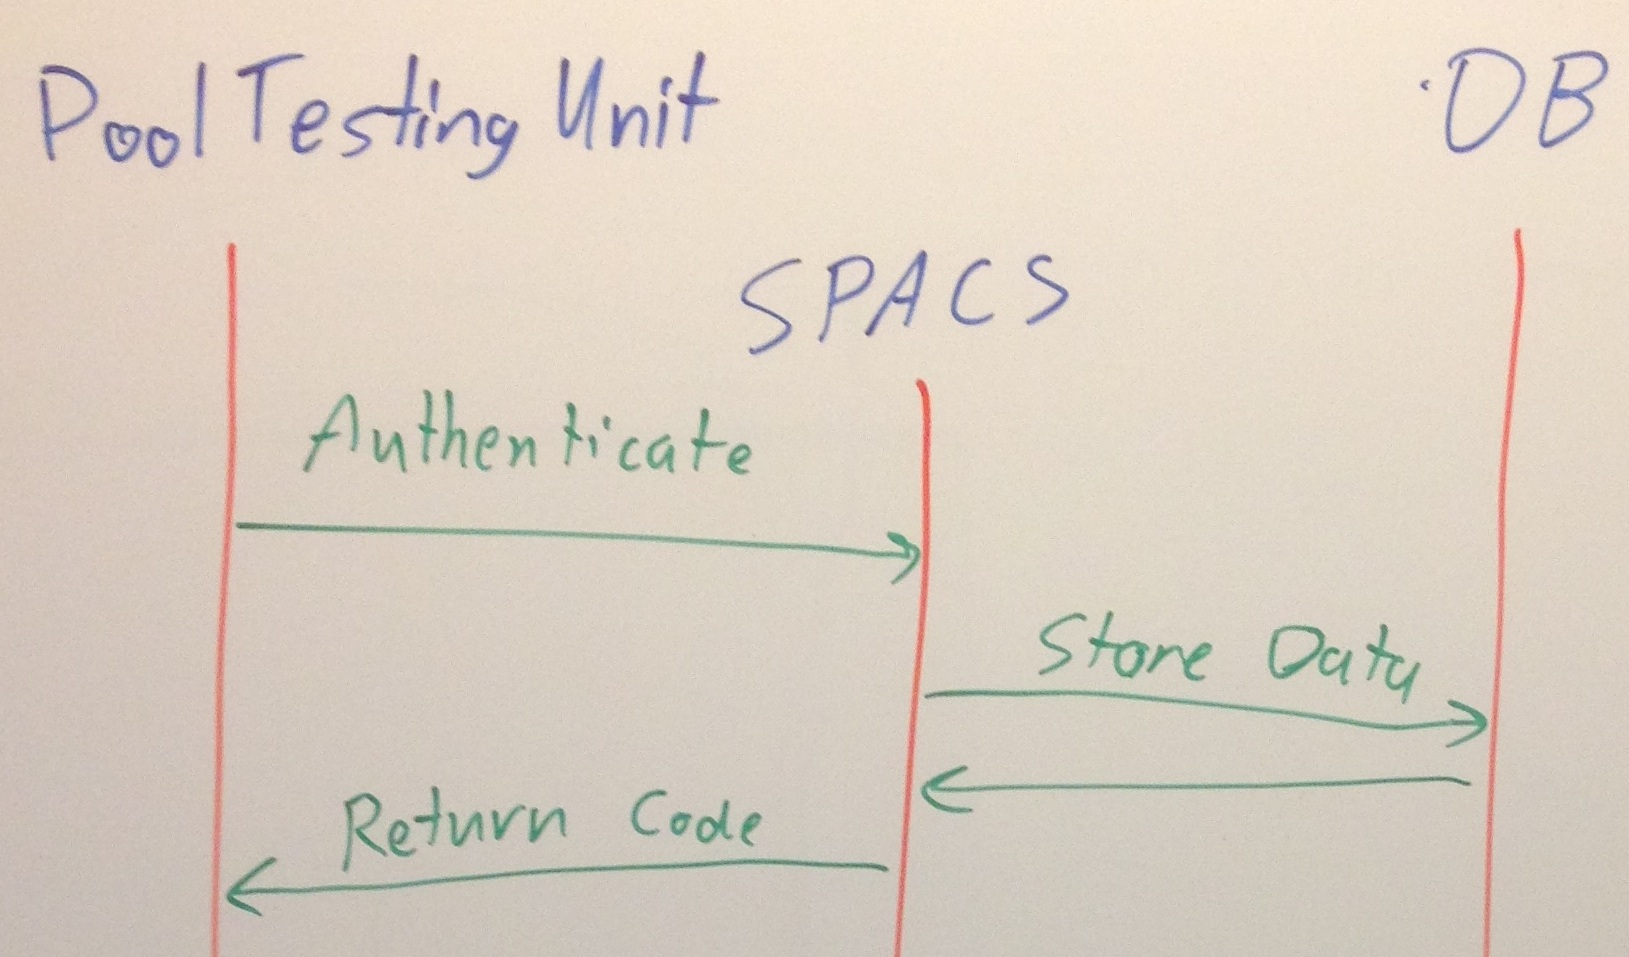
\includegraphics[width=14cm]{images/regular_update}
\end{center}
\end{figure}
\FloatBarrier

\subsection{urgent\_update}
\par
The urgent update differs to the regular update only by the PTUUpdate object sending off an email to the PoolOwner and PoolShopAdmin after the data is saved to the database.

\begin{figure}[!ht]
\begin{center}
	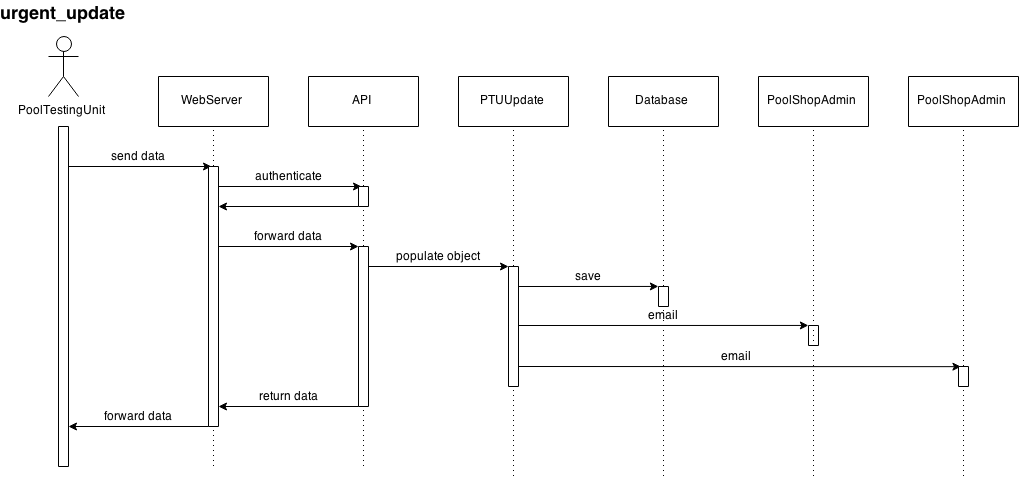
\includegraphics[width=14cm]{images/urgent_update}
\end{center}
\end{figure}
\FloatBarrier

\subsection{generate\_report}
\par
The ReportGenerator is started up by the Scheduler. It pulls in all the pools that need reports generated. These pools then pull in the information needed for the report. The ReportGenerator formats these nicely, then sends them off to the PoolOwner.

\begin{figure}[!ht]
\begin{center}
	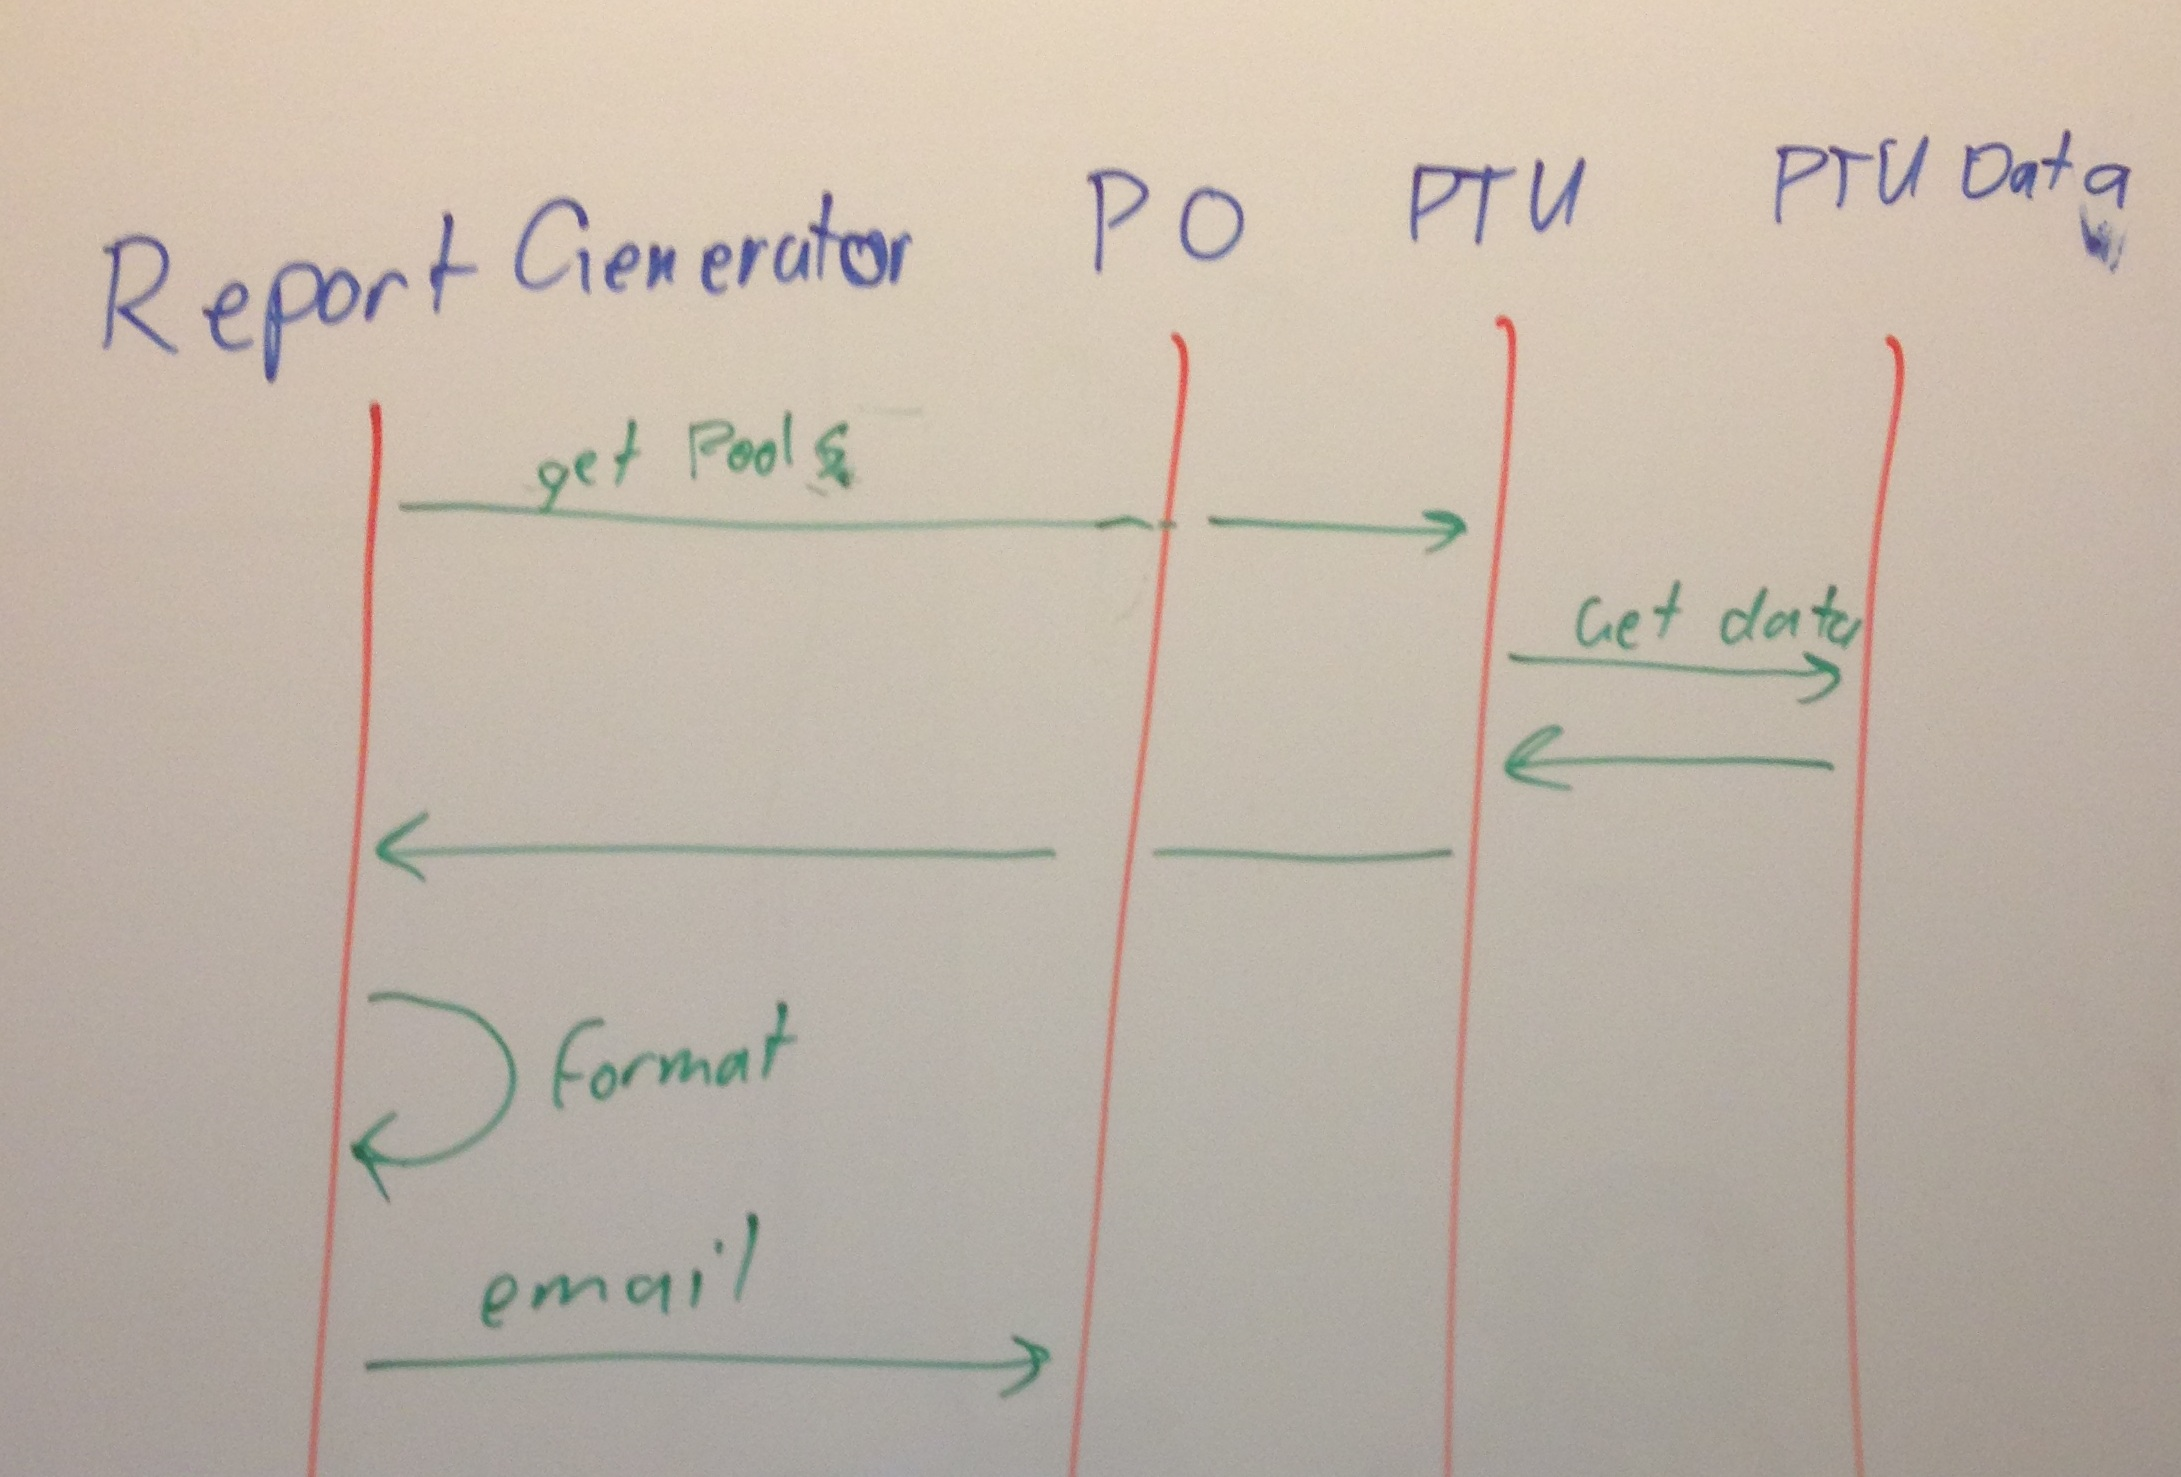
\includegraphics[width=14cm]{images/generate_report}
\end{center}
\end{figure}
\FloatBarrier

\subsection{edit\_pool\_shop\_admin}
\par
A PoolShopAdmin is edited by being sent the updated data via the web. This then gets parsed by the API which loads the PoolOwner out of the database. It's properties are then changed before being saved back to the database by the transaction bean. Information about the transaction is then returned to the user.

\begin{figure}[!ht]
\begin{center}
	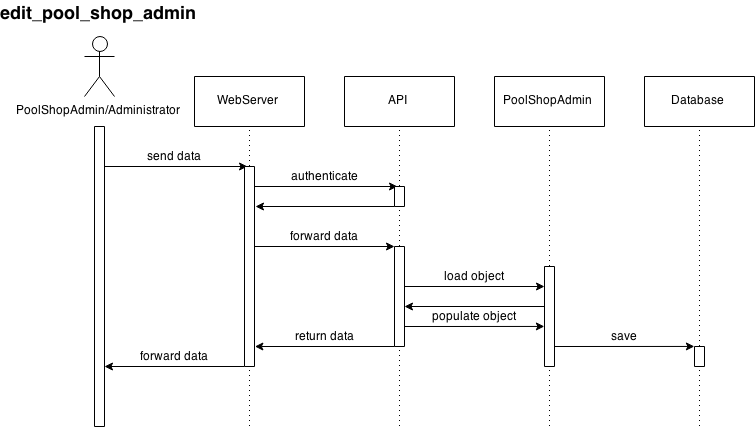
\includegraphics[width=14cm]{images/edit_pool_shop_admin}
\end{center}
\end{figure}
\FloatBarrier

\subsection{edit\_pool\_owner}
\par
Editing a PoolOwner is done in the same way as editing a PoolShopAdmin.

\begin{figure}[!ht]
\begin{center}
	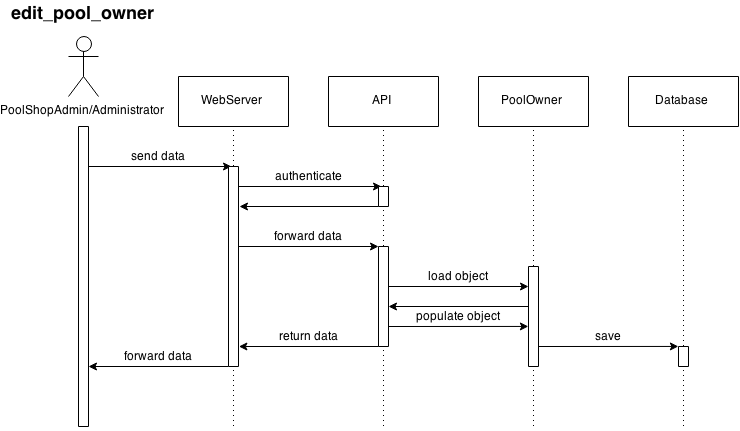
\includegraphics[width=14cm]{images/edit_pool_owner}
\end{center}
\end{figure}
\FloatBarrier